\documentclass [] {beamer} 
\usepackage[utf8]{inputenc}
\usepackage{booktabs, comment} 
\usepackage[absolute, overlay]{textpos} 
\usepackage{pgfpages}
\usepackage[font=footnotesize]{caption}
\useoutertheme{infolines} 

\definecolor{gold}{RGB}{254, 206, 0}

\setbeamercolor{title in head/foot}{bg=gold, fg=black}
\setbeamercolor{author in head/foot}{bg=myuniversity}
\setbeamertemplate{page number in head/foot}{}
\usepackage{csquotes}


\usepackage{amsmath}
\usepackage[makeroom]{cancel}


\usepackage{textpos}

\usepackage{tikz}

\usetheme{Madrid}
\definecolor{myuniversity}{RGB}{0, 85, 150}
\usecolortheme[named=myuniversity]{structure}
\usepackage{tikz}


\title[Online Application Forms]{Online Application Forms}
\subtitle{}
\institute[]{Department of Computer Science  and Engineering\\ Indian Institute of Technology Bombay}
\titlegraphic{
\includegraphics[height=2.5cm]{logo.png}}
\author[Balbir Singh]{
	Balbir Singh (R.N: 22M0747)\\Aniket Jadhav (R.N: 22M0817)}


\date{November 2022}

\begin{document}

\begin{frame}
\maketitle
\end{frame}


%%%%%%%%%%%%%%%%%%%%%%%%%%%%
\logo{
\includegraphics[scale=0.08]{logo.png}~%
}


%%%%%%%%%%%%%%%%%%%%%%%%%%



\begin{frame}
\frametitle{Table of Contents}
\tableofcontents
\end{frame}

\section{Description}
\begin{frame}{Description}
\begin{itemize}
 
\subsection{About Project}

    \item To provide a web application interface to students to fill application forms for the various programs in the IITB, online instead of offline.
    \item Students need to fill the form online and then submit to required authority.
    \item Application forms made online are available in the IITB website : 
    \href[pdfnewwindow=true]{https://www.iitb.ac.in/newacadhome/downloadForms/}{\beamergotobutton{Application Forms for various Programmes in IIT Bombay}}
    
\end{itemize}
\end{frame}

\subsection{Existing System}

\begin{frame}{Existing System}   
\begin{itemize}
    \item In Existing system students have to download Application form for various programs available and have to fill it manually and then submit offline.
    \item  This process is tedious and wastes lots of time for students as well as administration staff.
    \item Making application forms for different services available totally online will help both students as well as issuing authorities.
\end{itemize}
\end{frame}

\section{What did we achieve}
\begin{frame}{What did we achieve}


We have converted all the following offline forms to online.

\begin{columns}
    \begin{column}{0.48\textwidth}
\begin{itemize}
    \item Undertaking Forms
    \begin{itemize}
        \item \href{https://www.iitb.ac.in/newacadhome/UndertakingformGATE2022.pdf }{\beamergotobutton{GATE}}
        \item \href[pdfnewwindow=true]{https://www.iitb.ac.in/newacadhome/Undertakingform2021CEED.pdf}{\beamergotobutton{CEED}}
        
            
    \end{itemize}
    \item \href{https://www.iitb.ac.in/newacadhome/Withdrawalform.pdf}{\beamergotobutton{Withdrawal Form:}}
    \item \href{https://www.iitb.ac.in/newacadhome/Bonafidenew.pdf}{\beamergotobutton{Bonafide}}

    \item
    \href{https://www.iitb.ac.in/newacadhome/Reexamnewform.pdf}{\beamergotobutton{Re-Examination}}
\end{itemize}

    \end{column}
    \begin{column}{0.48\textwidth}
\begin{itemize}
    \item Successful Register and login of a user
    \item Email verification using OTP and Forget Password
4 Forgot password
\end{itemize}
    \end{column}
\end{columns}
\begin{columns}
    \begin{column}{0.48\textwidth}
        \textbf{Technology Learned }
        \begin{itemize}
            \item Django
            \item[*] Python
            \item[*] PostgreSQL
            \item[*] Latex
        \end{itemize}
    \end{column}
    \begin{column}{0.48\textwidth}
        \begin{itemize}
            \item HTML
            \item CSS
            \item JavaScript
            
            \item[*] IDE-- VSCode
            \item[*] git
            
        \end{itemize}
    \end{column}
    
\end{columns}

    
\end{frame}



\section{Future work pending}
\begin{frame}{Future work pending (Future Scope/Updation)}
\subsection{V1.5}
\begin{block}{Version 1.5:}
To write the application form data and PDF generated into database.
\end{block}
\subsection{V2.0}
\begin{block}{Version 2.0:}
\begin{itemize}
    \item As data of students are already available with the IITB , so instead of taking all information from students, students need to provide their LDAP ID (Roll. No.) and all information is fetched from the central repository.
    \item  E.g  Declaration form , students need to provide LDAP id all other information will filled automatically.
\end{itemize}

\end{block}
\end{frame}
\subsection{V3.0}
\begin{frame}{Version 3.0:}

\begin{block}{Version 3.0}
 \begin{itemize}
     \item   Student need not go to required authority for verification , the web application will send the request to verified authority online and they will verified internally.
     \item
     E.g for Institute Bonafide certificate, student need to provide roll no. only, Application (student information will automatically fetch from IITB records from version 2.0) request will be sent to academic office and academic office internally verified and provide the certificate online to the students.
     
 \end{itemize}
\end{block}

\end{frame}





\section{High level documentation of directories, files, main libraries/functions}

\begin{frame}{High level documentation of directories, files, main libraries/functions}

\subsection{Directory Structures}
\textbf{Directory Structures}
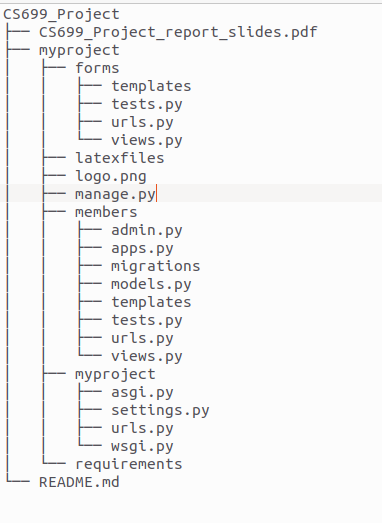
\includegraphics[width=2in]{directory.png}
\end{frame}

\subsection{Libraries Used}
\begin{frame}{Libraries Used}

\begin{itemize}
    \item django library   - basic webapp functionality
    \item os library - remove unneccessary files
    \item subprocess library - create subprocess to create latex to pdf
    \item pdflatex library - create latex to pdf document
    \item random library - generate random number for otp varification
\item mailjet library - send mail to desired users emailid using api and its services
\item models library - to create and use database according to djanago requirements
\item HttpResponse, HttpResponseRedirect -  send return response to webapp 
\item FileResponse - send file as response to webapp/browser
\item template loader - load html template from html files to render at browser
\end{itemize}


 
\end{frame}


\subsection{Functionality Implemented}
\begin{frame}{Functionality Implemented}
\begin{enumerate}
    \item Registration
    \item Login
    \item Email verification using OTP
    \item Forgot password
    \item Pdf forms creation from latex documents
    \begin{enumerate}
        \item Undertaking
        \item Withdrawal
        \item Re-examination.
        \item Bonafide

    \end{enumerate}
    \item Download Application pdf after creation.
\end{enumerate}







\end{frame}



% \section{High level documentation of any algorithms used}
% \begin{frame}{High level documentation of any algorithms used}

% \end{frame}

\section{Compilation and Running instructions}
\begin{frame}{Compilation and Running instructions}

\begin{enumerate}
    \item Install Required Packages
    \item Setup database
    \item Activate virtual environment
    \item Install more packages i.e pip install Django psycopg2
    \item Database Configuration
    \item Change ALLOWEDHOSTS in settings.py
    \item Make migrations and setup
    \item run python manage.py runserver 0.0.0.0:8000
    \item access via browser http://server-domain-or-IP:8000
\end{enumerate}


\end{frame}


\begin{frame}
  \center{\huge{\textbf{Thank You}}
}
\end{frame}

\end{document}
